
\documentclass{article}
\usepackage[utf8]{inputenc}
\usepackage{amstext}
\usepackage{amsmath}
\usepackage{amsfonts}
\usepackage{graphicx}
\usepackage[margin=1in, paperwidth=8.5in, paperheight=11in]{geometry}
\usepackage{gensymb}
\usepackage{indentfirst}
\usepackage{textcomp}
\usepackage{upgreek }
\usepackage{siunitx}
\usepackage{enumitem}
\usepackage{epstopdf}
\epstopdfsetup{update} % only regenerate pdf files when eps file is newer

\usepackage[american]{circuitikz}

\title{Circuits Postlab 9}
\author{Byron Wasti}
\date{April 2017}

\begin{document}
\maketitle

The schematic for the rail-to-rail common-mode input range and rail-to-rail output swing differential amplifier is shown in Figure \ref{fig:1}. The step responses from near the lower rail, near the center of the operating range, and from near the upper rail, are shown in Figures \ref{fig:2}, \ref{fig:3}, \ref{fig:4} respectively.

As seen in the step-response figures, the time constant of the circuit is higher near the rails than it is in the center of the input range.

\begin{figure}[ht!]
    \centering
    \includegraphics[width=\textwidth]{../schematic}
    \caption{Schematic for the differential amplifier in LTSpice}
    \label{fig:1}
\end{figure}

\begin{figure}[ht!]
    \centering
    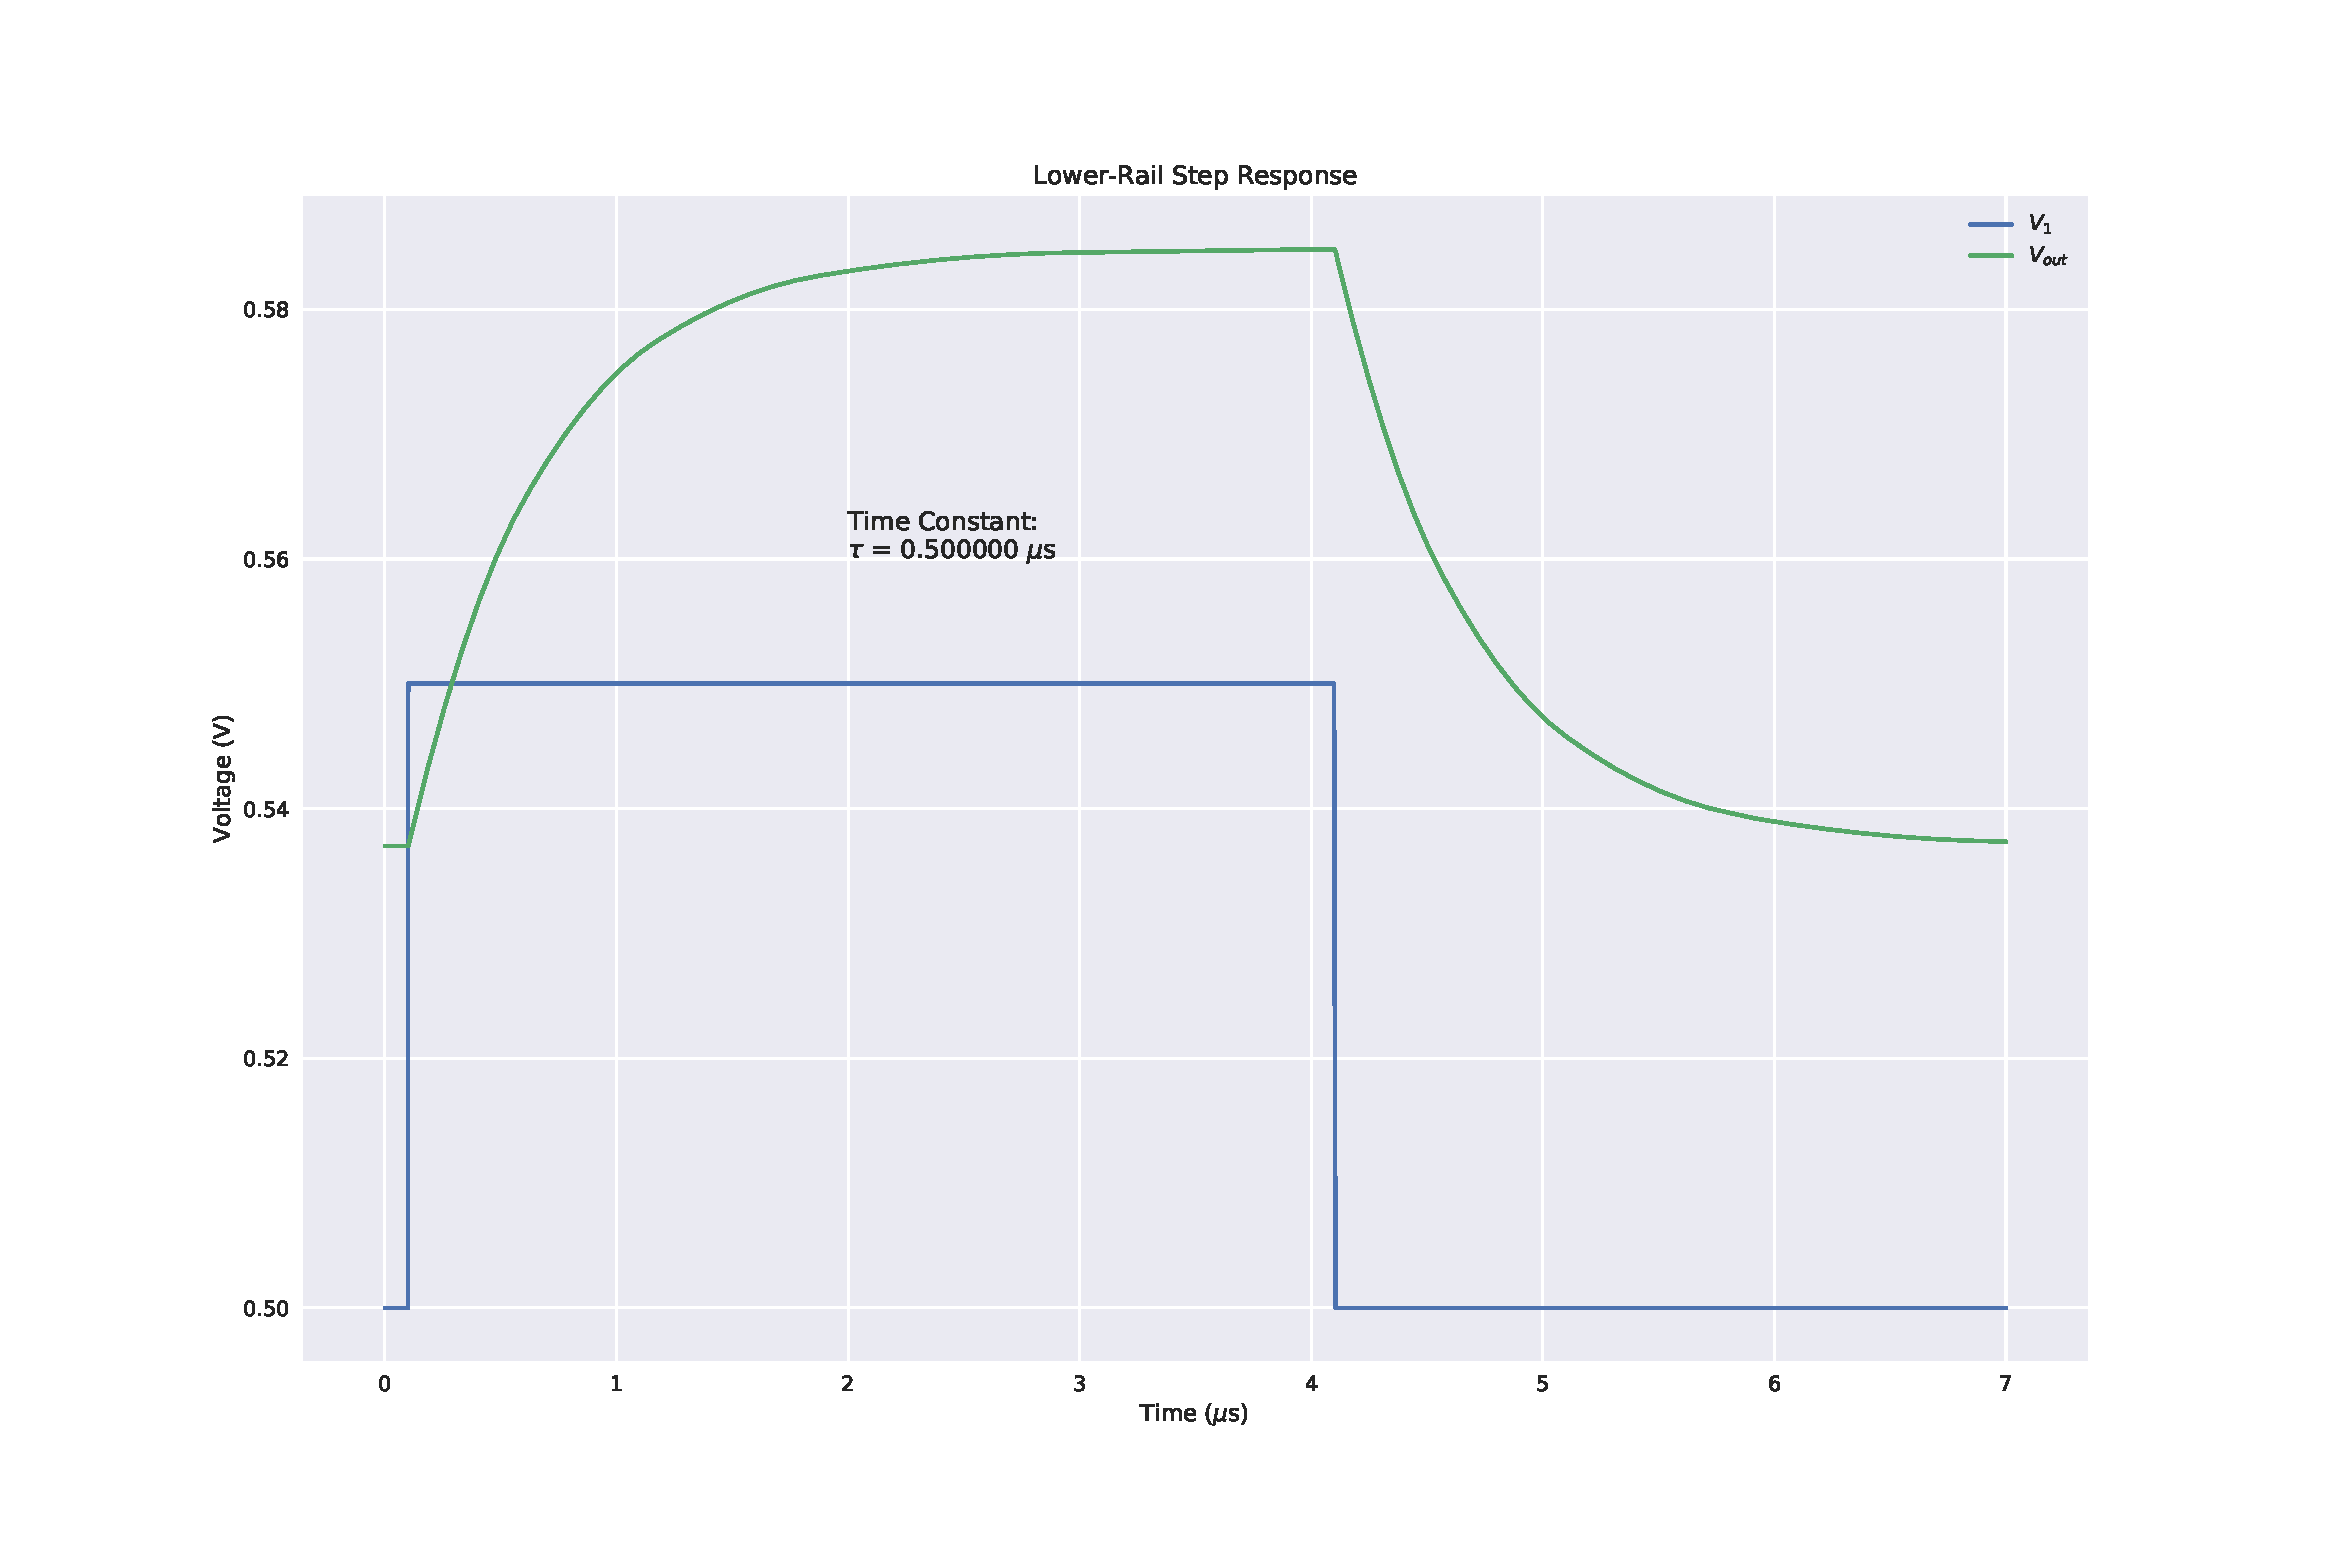
\includegraphics[width=\textwidth]{low}
    \caption{Step-response near the lower-rail of the differential amplifier}
    \label{fig:2}
\end{figure}

\begin{figure}[ht!]
    \centering
    \includegraphics[width=\textwidth]{middle}
    \caption{Step-response at the center of the input range of the differential amplifier}
    \label{fig:3}
\end{figure}

\begin{figure}[ht!]
    \centering
    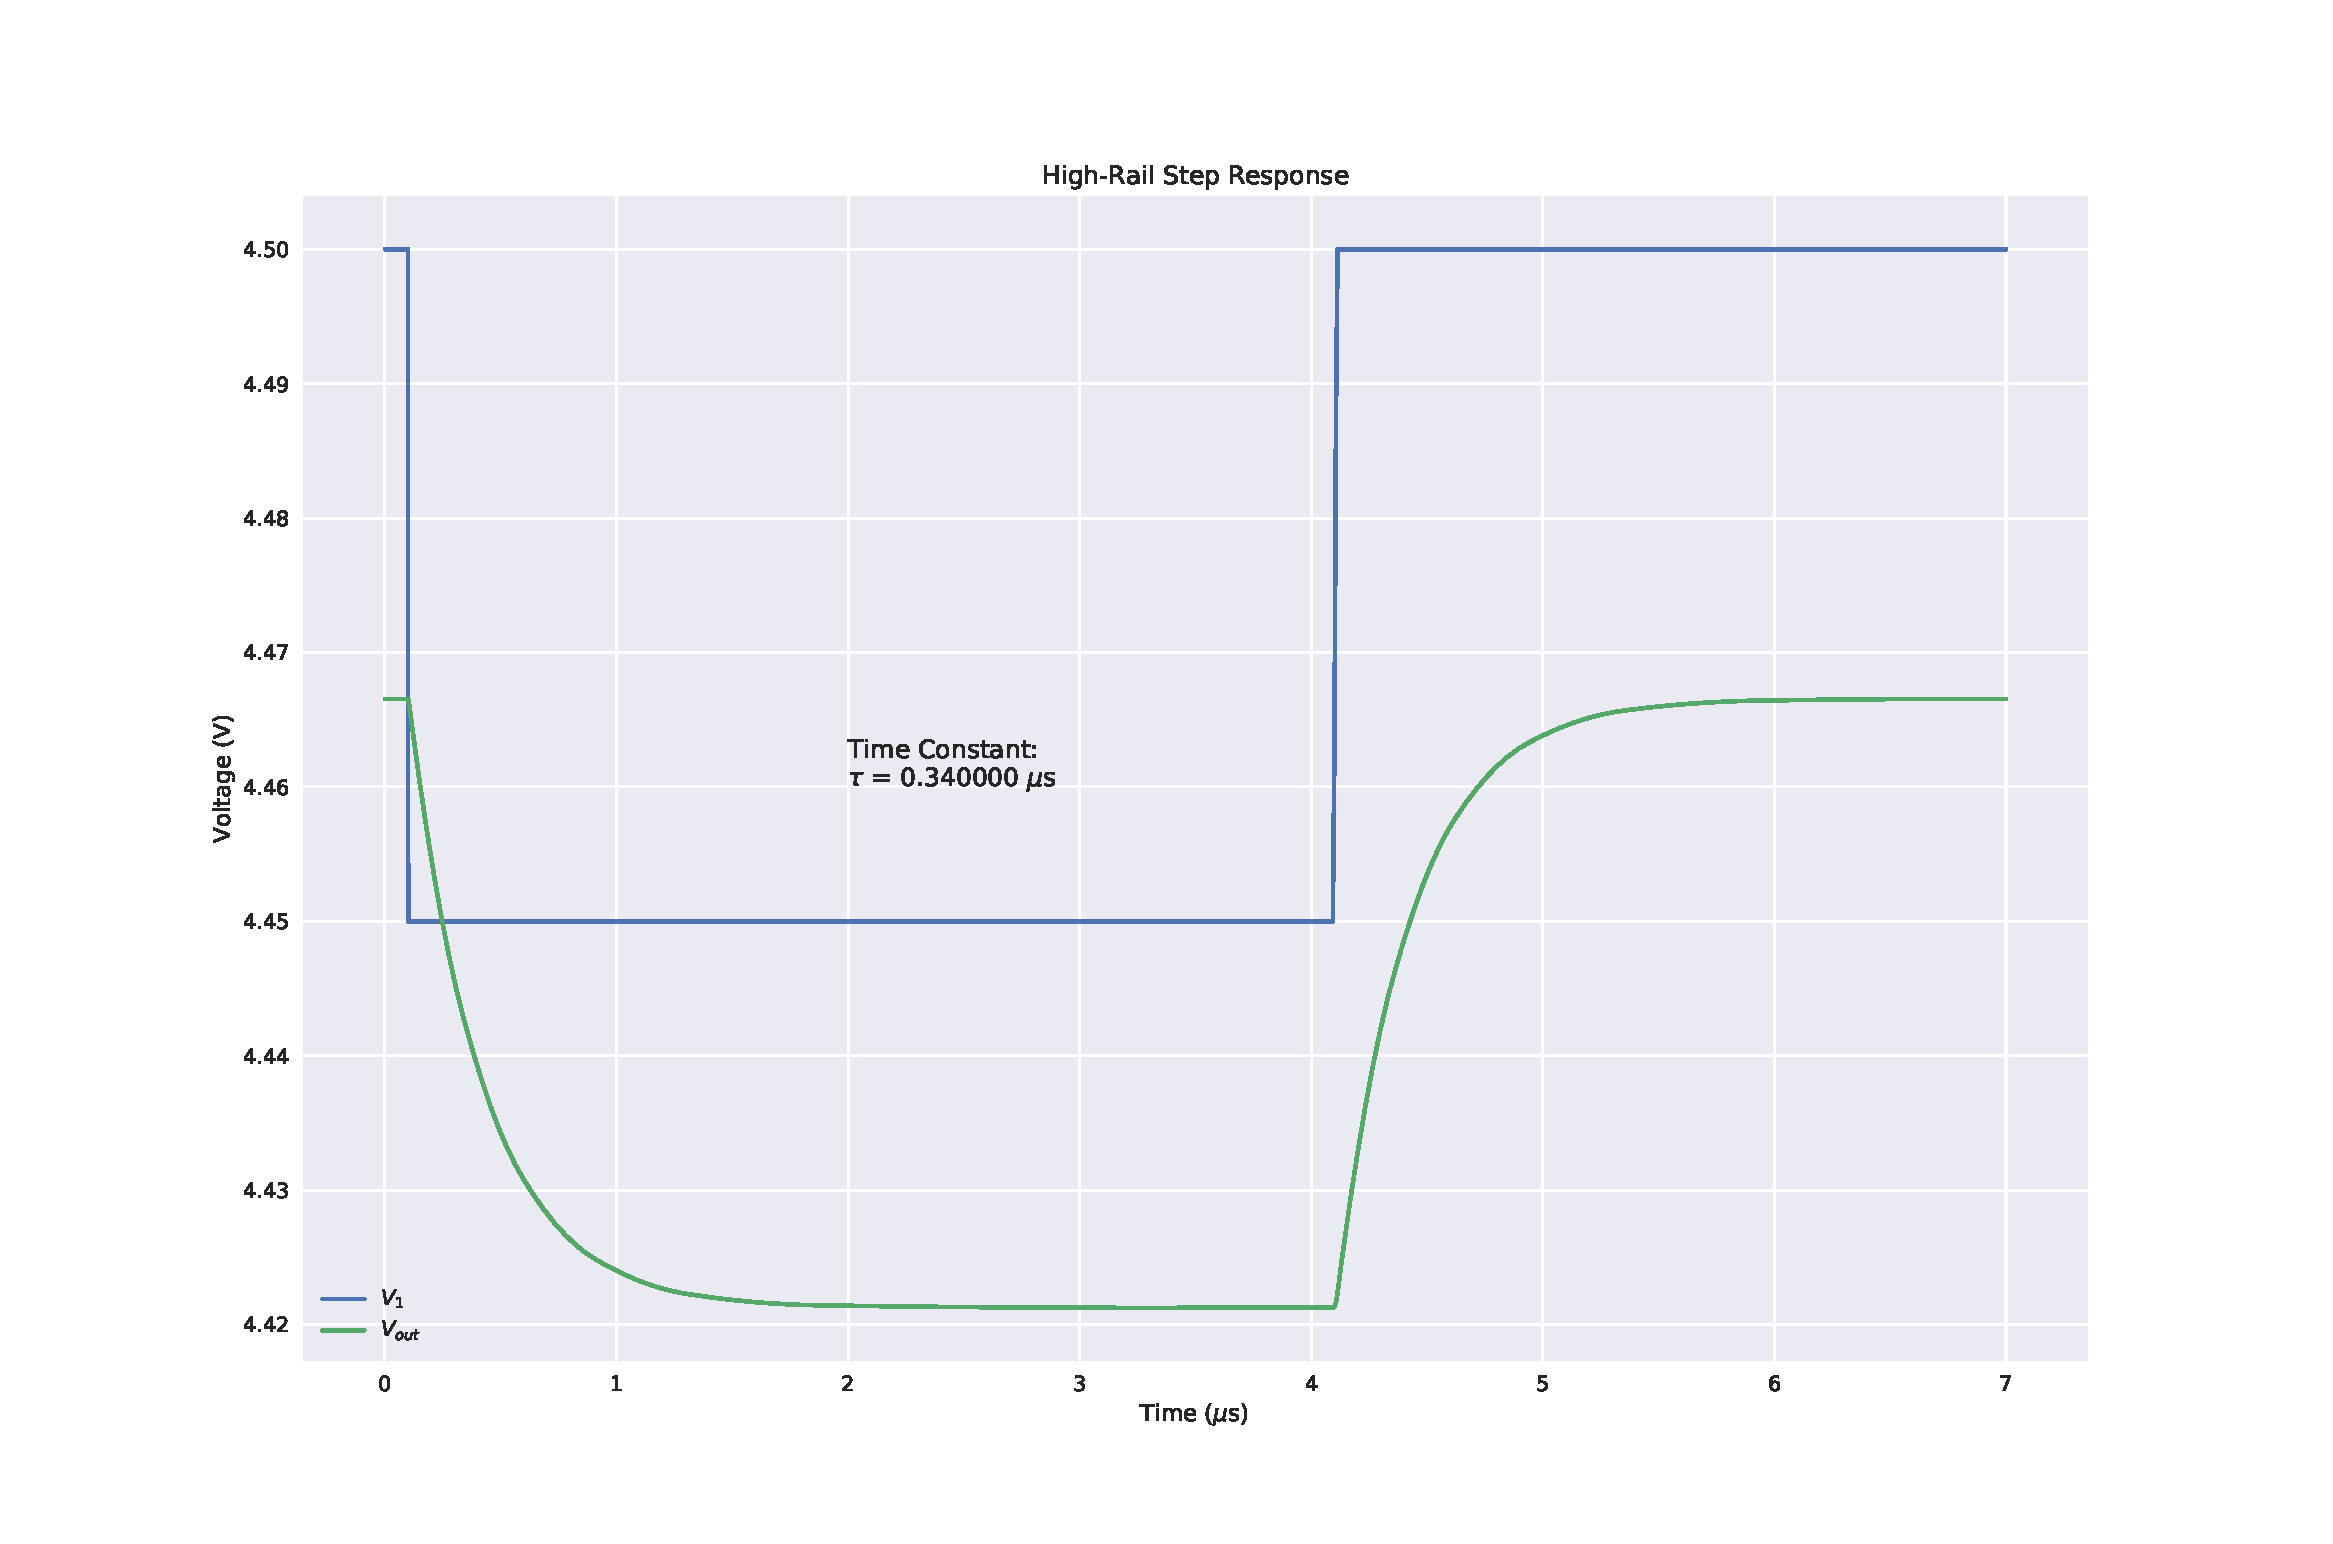
\includegraphics[width=\textwidth]{high}
    \caption{Step-response near the upper-rail of the differential amplifier}
    \label{fig:4}
\end{figure}

\end{document}
